%prescription_latex.tex

\documentclass{article}
\usepackage[utf8]{inputenc}
\usepackage[spanish]{babel}
\usepackage[T1]{fontenc}
\usepackage{textcomp}
\usepackage{graphicx}
\usepackage{eso-pic}
\usepackage{ifthen}
\usepackage[abs]{overpic}
\usepackage{pict2e,xcolor,varwidth}
\usepackage{color}
\usepackage{layout}
%\usepackage{tikz}
%\usepackage{relsize}
\usepackage{etoolbox}
\usepackage[paperwidth=27.94cm, paperheight=21.59cm, left=0.0cm,right=0.0cm,top=0.0in,bottom=0.0in,headheight=0in,headsep=0pt,footskip=120pt]{geometry}
% Check parameters in: https://en.wikibooks.org/wiki/LaTeX/Page_Layout
%{# Define where latex finds images #}
{{ latex_graphics_path }}
%\setmainfont{Arial}
%\usepackage{fancyhdr}
\usepackage{uarial}
%\usepackage[scaled]{uarial}
\usepackage{transparent}
\usepackage[protrusion=true,expansion=true]{microtype}
\usepackage{calc}
\usepackage{verbatim}
\makeatletter
\g@addto@macro\@verbatim\small
\makeatother 
\usepackage{xcolor}

\usepackage{lmodern}
%\fontfamily{lmss}\selectfont
\usepackage[utf8]{inputenc}
%\usepackage{unixode}


\begin{document}
\fontfamily{lmss}\selectfont
    % Include Background in ./prescript/media/media/template_v1.pdf
    % \AddToShipoutPictureBG{\ifthenelse{\isodd{\value{page}}}{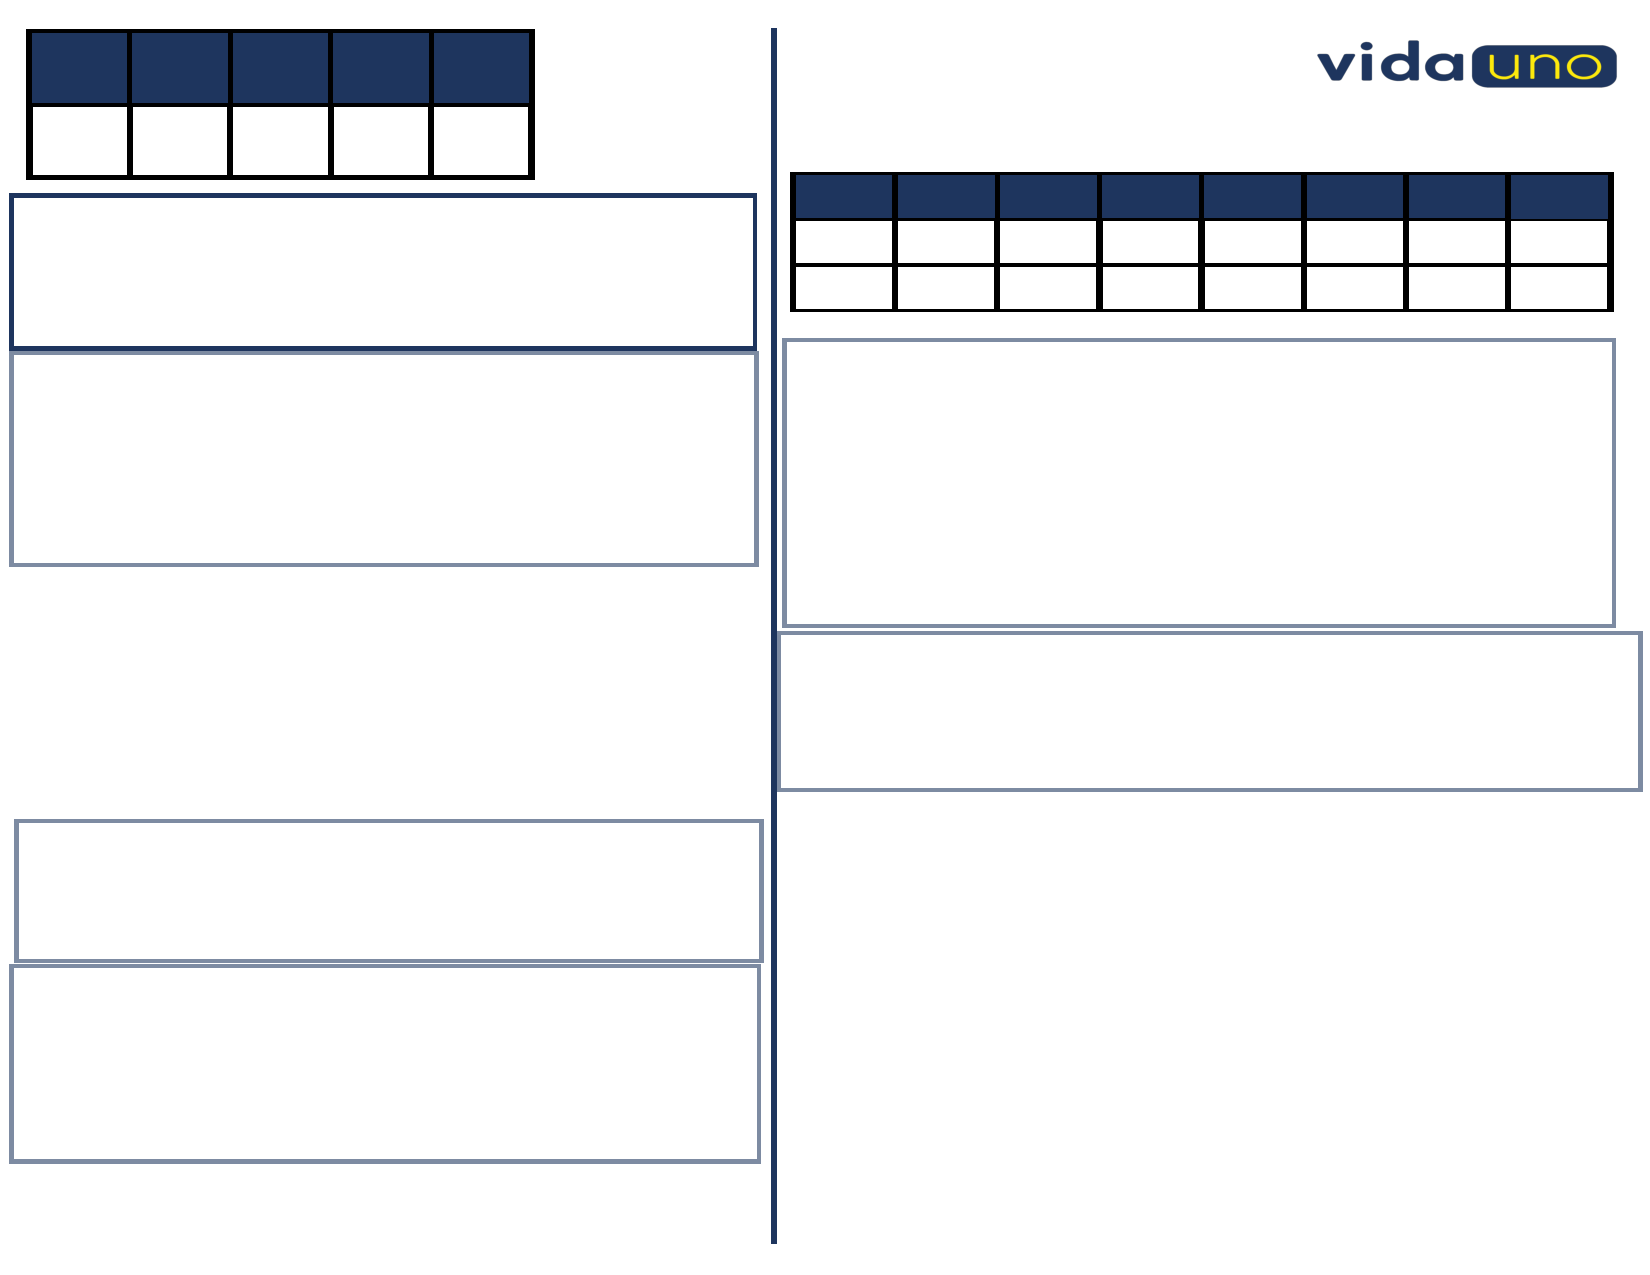
\includegraphics{laam_template}}{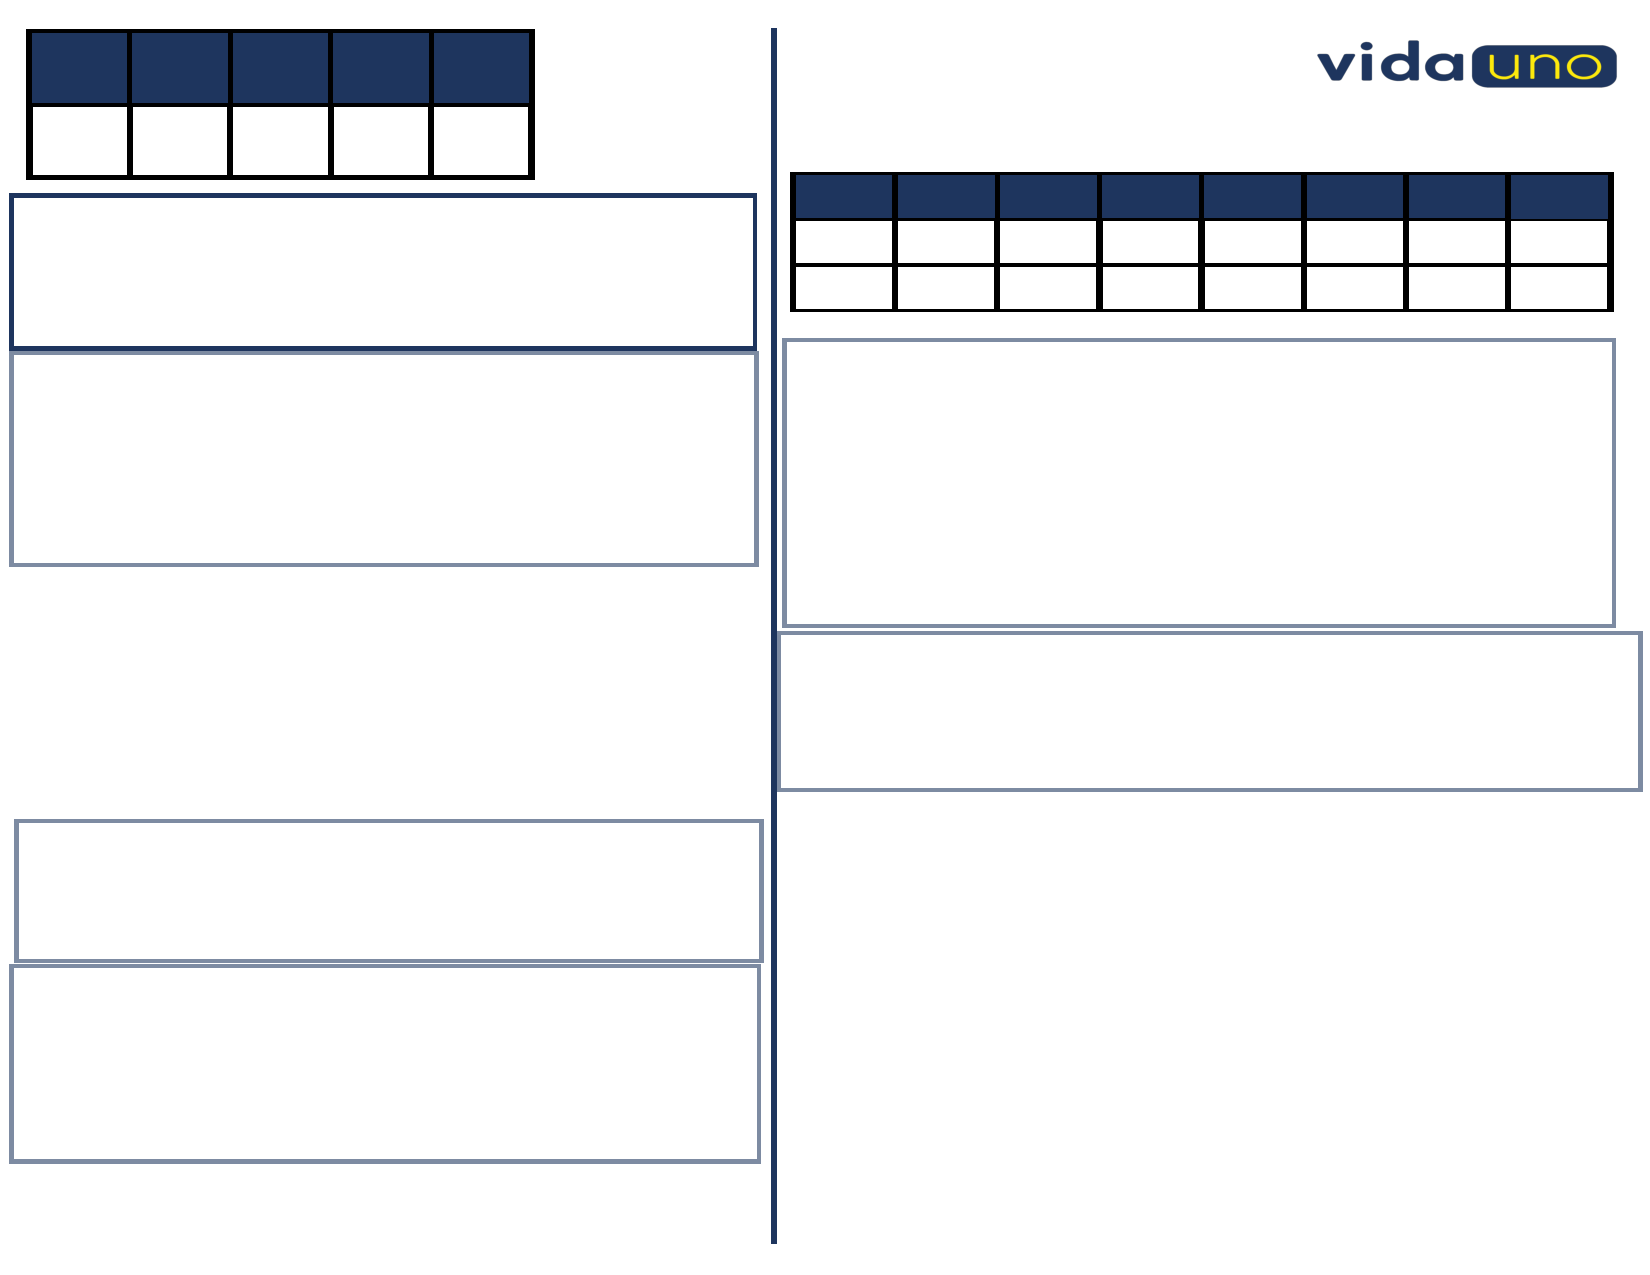
\includegraphics{laam_template}}}
    % Define page content
    %\textsf{\large{
    %\begin{changemargin}{1.5cm}{1.2cm}
        %\begin{enumerate}
            %{{ all_medications }}
            %bla!
        %\end{enumerate}
    %         \put(1,1){\parbox[t]{3cm}{\textsf{\large{
    %    \textbf{Consulta \#:} {{ content.id }}
    % }
    % }}}
        % Indicaciones Extra
        % \begin{enumerate}
        %     \textbf{Indicaciones Extra: \\ } {{ all_medications }}
        % \end{enumerate}
    %\end{changemargin}
    %}}
    % \begin{picture}(1,0.77272727)%
    %     %Consulta    
    % \put(200,0){\parbox[t]{3cm}{\textsf{\large{
    %    \textbf{{ content.id }}
    % }
    % }}}
    % \end{picture}
% \begingroup%
%   \makeatletter%
%   \providecommand\color[2][]{%
%     \errmessage{(Inkscape) Color is used for the text in Inkscape, but the package 'color.sty' is not loaded}%
%     \renewcommand\color[2][]{}%
%   }%
%   \providecommand\transparent[1]{%
%     \errmessage{(Inkscape) Transparency is used (non-zero) for the text in Inkscape, but the package 'transparent.sty' is not loaded}%
%     \renewcommand\transparent[1]{}%
%   }%
%   \providecommand\rotatebox[2]{#2}%
%   \newcommand\scaleInNode[1][1]{\tikzset{execute at begin node={\normalsize\larger[#1]}}}
%   \newcommand*\fsize{\dimexpr\f@size pt\relax}%
%   \newcommand*\lineheight[1]{\fontsize{\fsize}{#1\fsize}\selectfont}%
%   \ifx\svgwidth\undefined%
%     \setlength{\unitlength}{792bp}%
%     \ifx\svgscale\undefined%
%       \relax%
%     \else%
%       \setlength{\unitlength}{\unitlength * \real{\svgscale}}%
%     \fi%
%   \else%
%     \setlength{\unitlength}{\svgwidth}%
%   \fi%
%   \global\let\svgwidth\undefined%
%   \global\let\svgscale\undefined%
%   \makeatother%
%   \begin{picture}(1,0.77272727)%
%     \lineheight{1}%
%     \setlength\tabcolsep{0pt}%
%     \put(0,0){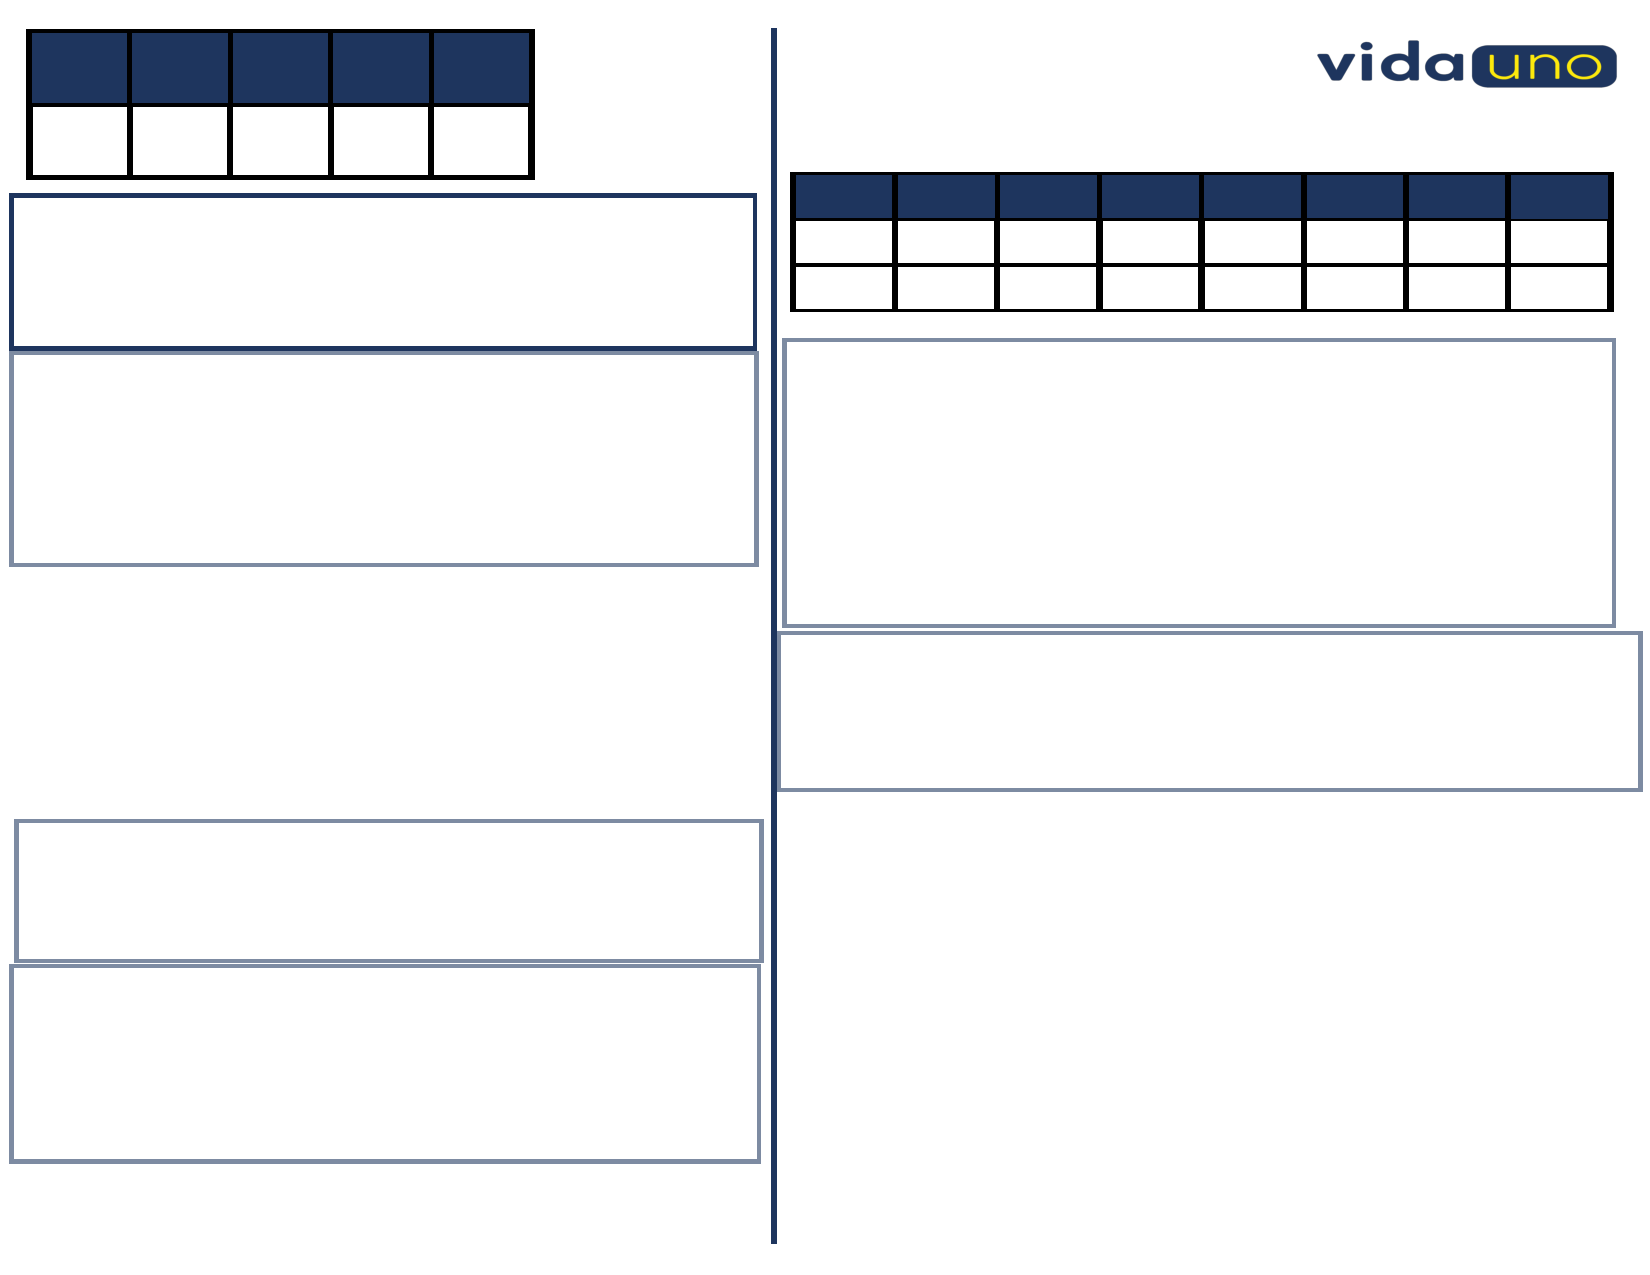
\includegraphics[width=\unitlength,page=1]{laam_template}}%

%     % \put(0.01140896,0.54355203){\parbox[t]{3cm}{\textsf{\large{
%     %    \textbf{Consulta \#:} {{ content.id }}
%     % }
%     % }}}
%     % \put(0.01140896,0.54355203){\color[rgb]{0.11764706,0.20784314,0.36862745}\makebox(0,0)[lt]{\lineheight{1.25}\smash{\begin{tabular}[t]{l}\textbf{Paciente desconocido {{content.id}} }\end{tabular}}}}%
% 	\put(0.42718184,0.73912713){\color[rgb]{0,0,0}\makebox(0,0)[lt]{\lineheight{1.25}\smash{\begin{tabular}[t]{l}\textit{ {{content.id}} }\end{tabular}}}}%
%    	\put(0.42718184,0.72336542){\color[rgb]{0,0,0}\makebox(0,0)[lt]{\lineheight{1.25}\smash{\begin{tabular}[t]{l}\textit{ {{content.service_unit }} }\end{tabular}}}}%
%     \put(0.3690564,0.69389968){\color[rgb]{0,0,0}\makebox(0,0)[lt]{\lineheight{1.25}\smash{\begin{tabular}[t]{l}\textit{ {{content.service_unit_type}} }\end{tabular}}}}%
%     \put(0.39254546,0.6775768){\color[rgb]{0,0,0}\makebox(0,0)[lt]{\lineheight{1.25}\smash{\begin{tabular}[t]{l}\textit{ {{content.service_unit_plate}} }\end{tabular}}}}%

%   \end{picture}%
% \endgroup%

\begin{figure}
  \centering
  \def\svgwidth{\columnwidth}
  %\input{paperless_template_6.pdf_tex}

\begingroup%
  \makeatletter%
  \providecommand\color[2][]{%
    \errmessage{(Inkscape) Color is used for the text in Inkscape, but the package 'color.sty' is not loaded}%
    \renewcommand\color[2][]{}%
  }%
  \providecommand\transparent[1]{%
    \errmessage{(Inkscape) Transparency is used (non-zero) for the text in Inkscape, but the package 'transparent.sty' is not loaded}%
    \renewcommand\transparent[1]{}%
  }%
  \providecommand\rotatebox[2]{#2}%
  \newcommand*\fsize{\dimexpr\f@size pt\relax}%
  \newcommand*\lineheight[1]{\fontsize{\fsize}{#1\fsize}\selectfont}%
  \ifx\svgwidth\undefined%
    \setlength{\unitlength}{782.27360219bp}%
    \ifx\svgscale\undefined%
      \relax%
    \else%
      \setlength{\unitlength}{\unitlength * \real{\svgscale}}%
    \fi%
  \else%
    \setlength{\unitlength}{\svgwidth}%
  \fi%
  \global\let\svgwidth\undefined%
  \global\let\svgscale\undefined%
  \makeatother%
  \begin{picture}(1,0.77245213)%
    \lineheight{1}%
    \setlength\tabcolsep{0pt}%
    \put(0,0){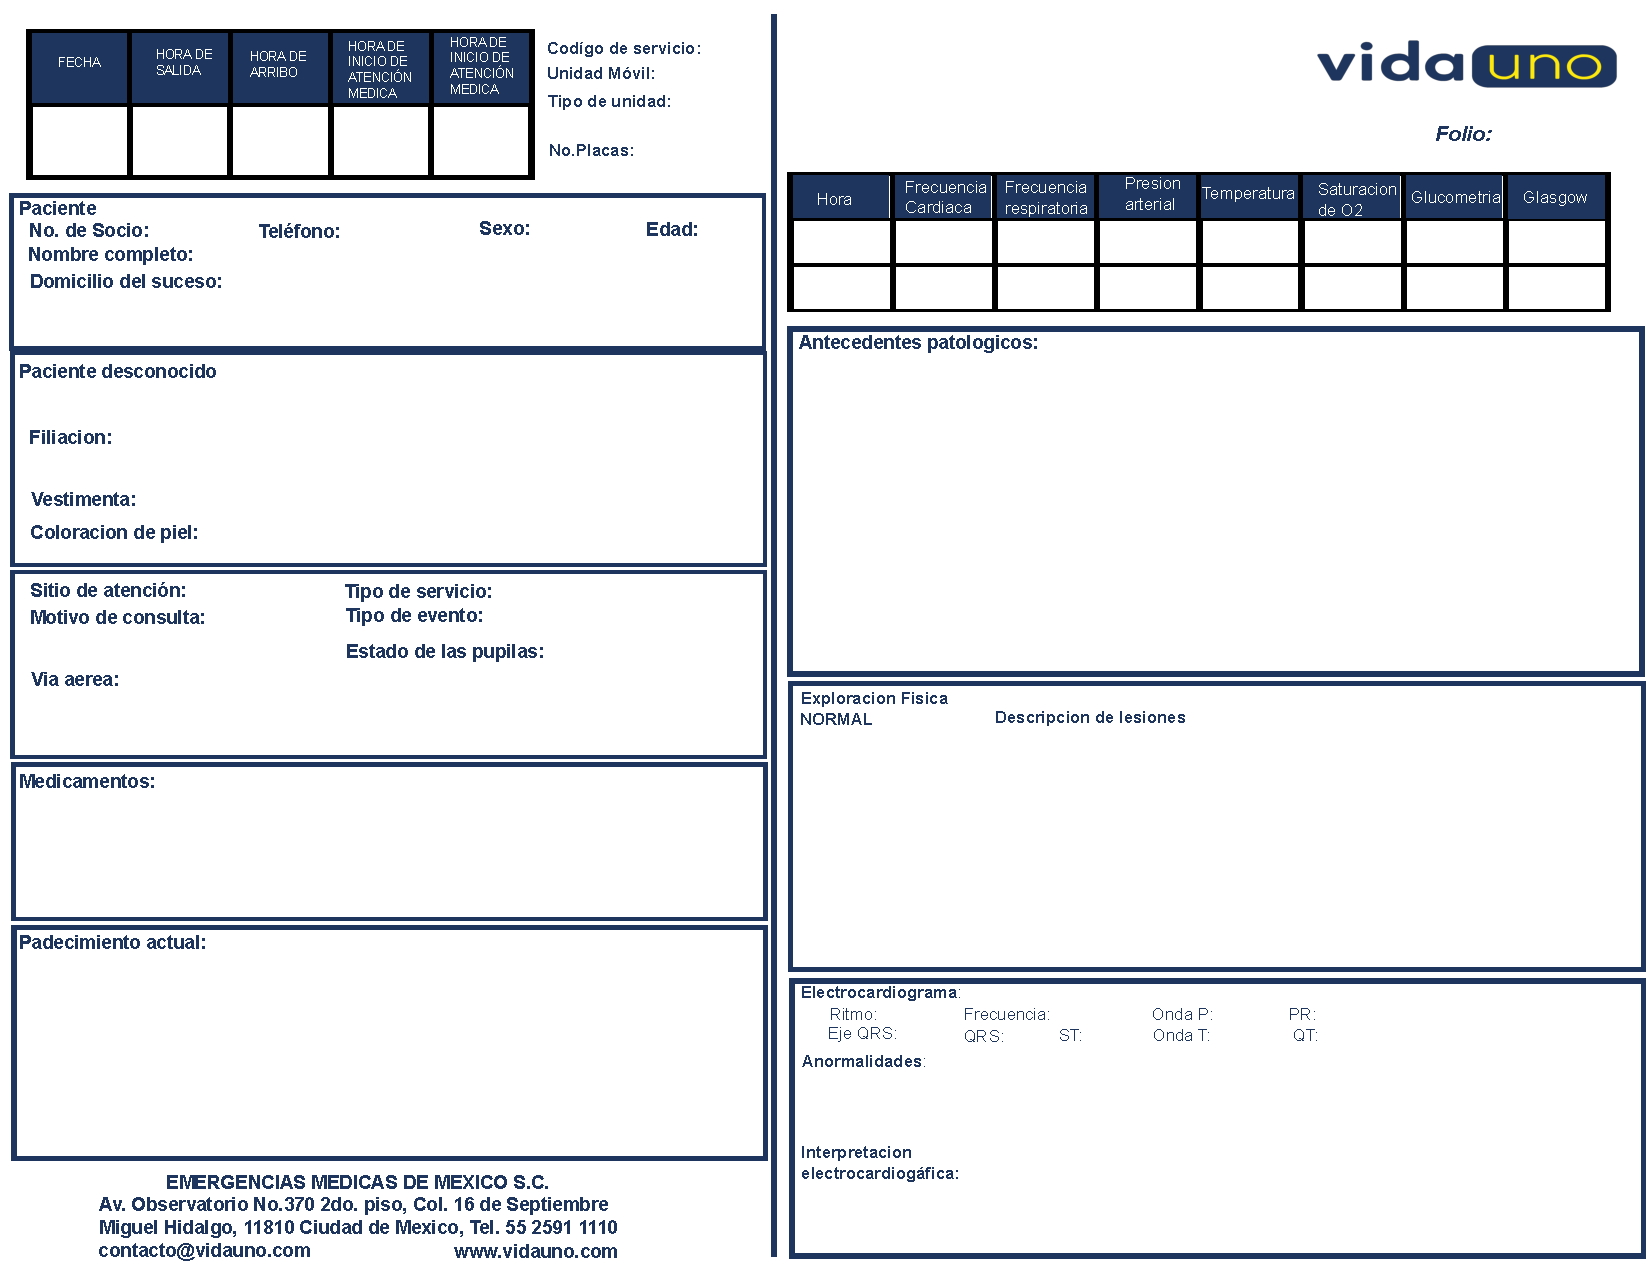
\includegraphics[width=\unitlength,page=1]{paperless_template_page_1}}%

    \put(0.42638971,0.73960084){\color[rgb]{0.11764706,0.20784314,0.36862745}\makebox(0,0)[lt]{\lineheight{1.25}\smash{\begin{tabular}[t]{l}\fontfamily{lmss}\selectfont {{content.service_code}}\end{tabular}}}}%
    \put(0.43014479,0.72364315){\color[rgb]{0.11764706,0.20784314,0.36862745}\makebox(0,0)[lt]{\lineheight{1.25}\smash{\begin{tabular}[t]{l}\fontfamily{lmss}\selectfont {{content.service_unit}}\end{tabular}}}}%
   	\put(0.33829987,0.69381105){\color[rgb]{0.11764706,0.20784314,0.36862745}\makebox(0,0)[lt]{\lineheight{1.25}\smash{\begin{tabular}[t]{l}\fontfamily{lmss}\selectfont {{content.service_unit_type}}\end{tabular}}}}%
    \put(0.39132267,0.67728521){\color[rgb]{0.11764706,0.20784314,0.36862745}\makebox(0,0)[lt]{\lineheight{1.25}\smash{\begin{tabular}[t]{l}\fontfamily{lmss}\selectfont {{content.service_unit_plate}}\end{tabular}}}}%

    %Paciente
    \put(0.09655761,0.62853648){\color[rgb]{0.11764706,0.20784314,0.36862745}\makebox(0,0)[lt]{\lineheight{1.25}\smash{\begin{tabular}[t]{l}\fontfamily{lmss}\selectfont {{content.erste_code}}\end{tabular}}}}%
    \put(0.20912356,0.62853648){\color[rgb]{0.11764706,0.20784314,0.36862745}\makebox(0,0)[lt]{\lineheight{1.25}\smash{\begin{tabular}[t]{l}\fontfamily{lmss}\selectfont {{content.patient_phone}}\end{tabular}}}}%
    \put(0.3268484,0.62853648){\color[rgb]{0.11764706,0.20784314,0.36862745}\makebox(0,0)[lt]{\lineheight{1.25}\smash{\begin{tabular}[t]{l}\fontfamily{lmss}\selectfont {{content.patient_gender}}\end{tabular}}}}%
    \put(0.42764439,0.62853648){\color[rgb]{0.11764706,0.20784314,0.36862745}\makebox(0,0)[lt]{\lineheight{1.25}\smash{\begin{tabular}[t]{l}\fontfamily{lmss}\selectfont {{content.patient_age}}\end{tabular}}}}%
    \put(0.12766308,0.61324599){\color[rgb]{0.11764706,0.20784314,0.36862745}\makebox(0,0)[lt]{\lineheight{1.25}\smash{\begin{tabular}[t]{l}\fontfamily{lmss}\selectfont {{content.patient_name}}\end{tabular}}}}%
    \put(0.02575936,0.58169366){\color[rgb]{0.11764706,0.20784314,0.36862745}\makebox(0,0)[lt]{\lineheight{1.25}\smash{\begin{tabular}[t]{l}\fontfamily{lmss}\selectfont {{content.patient_address}}\end{tabular}}}}%


    %Paciente desconocido
    \put(0.01999075,0.53033139){\color[rgb]{0.11764706,0.20784314,0.36862745}\makebox(0,0)[lt]{\lineheight{1.25}\smash{\begin{tabular}[t]{l}\fontfamily{lmss}\selectfont {{content.patient_unknow}}\end{tabular}}}}%
    \put(0.01999075,0.48794778){\color[rgb]{0.11764706,0.20784314,0.36862745}\makebox(0,0)[lt]{\lineheight{1.25}\smash{\begin{tabular}[t]{l}\fontfamily{lmss}\selectfont  {{content.patient_affiliations}}\end{tabular}}}}%
    \put(0.09106678,0.46594263){\color[rgb]{0.11764706,0.20784314,0.36862745}\makebox(0,0)[lt]{\lineheight{1.25}\smash{\begin{tabular}[t]{l}\fontfamily{lmss}\selectfont {{content.patient_clothes}}\end{tabular}}}}%
    \put(0.12588643,0.44615019){\color[rgb]{0.11764706,0.20784314,0.36862745}\makebox(0,0)[lt]{\lineheight{1.25}\smash{\begin{tabular}[t]{l}\fontfamily{lmss}\selectfont {{content.skin_color}}\end{tabular}}}}%

    %Padecimiento
    \put(0.0159714,0.1825995){\color[rgb]{0.11764706,0.20784314,0.36862745}\makebox(0,0)[lt]{\lineheight{1.25}\smash{\begin{tabular}[t]{l}\fontfamily{lmss}\selectfont {{content.current_condition}}\end{tabular}}}}%
    %\put(0.02265882,0.24439213){\color[rgb]{0.11764706,0.20784314,0.36862745}\makebox(0,0)[lt]{\lineheight{1.25}\smash{\begin{tabular}[t]{l}\fontfamily{lmss}\selectfont {{content.current_condition}}\end{tabular}}}}%

    %Generales
    \put(0.12027596,0.41209986){\color[rgb]{0.11764706,0.20784314,0.36862745}\makebox(0,0)[lt]{\lineheight{1.25}\smash{\begin{tabular}[t]{l}\fontfamily{lmss}\selectfont {{content.attention_place}} \end{tabular}}}}%
    \put(0.30209431,0.41082061){\color[rgb]{0.11764706,0.20784314,0.36862745}\makebox(0,0)[lt]{\lineheight{1.25}\smash{\begin{tabular}[t]{l}\fontfamily{lmss}\selectfont {{content.service_type}} \end{tabular}}}}%
    \put(0.30209431,0.39566916){\color[rgb]{0.11764706,0.20784314,0.36862745}\makebox(0,0)[lt]{\lineheight{1.25}\smash{\begin{tabular}[t]{l}\fontfamily{lmss}\selectfont {{content.event_type}} \end{tabular}}}}%
    \put(0.21257984,0.38532216){\color[rgb]{0.11764706,0.20784314,0.36862745}\makebox(0,0)[lt]{\lineheight{1.25}\smash{\begin{tabular}[t]{l}\fontfamily{lmss}\selectfont {{content.traumatics}} \end{tabular}}}}%
    \put(0.20991809,0.36213786){\color[rgb]{0.11764706,0.20784314,0.36862745}\makebox(0,0)[lt]{\lineheight{1.25}\smash{\begin{tabular}[t]{l}\fontfamily{lmss}\selectfont Ojo Izquierdo:{{content.pupil_state_left}}\end{tabular}}}}%
    \put(0.20991809,0.35077424){\color[rgb]{0.11764706,0.20784314,0.36862745}\makebox(0,0)[lt]{\lineheight{1.25}\smash{\begin{tabular}[t]{l}\fontfamily{lmss}\selectfont Ojo Derecho:  {{content.pupil_state_right}}\end{tabular}}}}%
    \put(0.016641,0.38301062){\color[rgb]{0.11764706,0.20784314,0.36862745}\makebox(0,0)[lt]{\lineheight{1.25}\smash{\begin{tabular}[t]{l}\fontfamily{lmss}\selectfont {{content.consultation_reason}}\end{tabular}}}}%
    %to_fix

    %Medicamentos (to_fix)
    %\put(0.0159714,0.27918911){\color[rgb]{0.11764706,0.20784314,0.36862745}\makebox(0,0)[lt]{\lineheight{1.25}\smash{\begin{tabular}[t]{l}\fontfamily{lmss}\selectfont {{ content.medications|truncatechars:20}}\end{tabular}}}}%

    %Antecedentes
    %Diabetes
    \put(0.48529688,0.5272494){\color[rgb]{0.11764706,0.20784314,0.36862745}\makebox(0,0)[lt]{\lineheight{1.25}\smash{\begin{tabular}[t]{l}\fontfamily{lmss}\selectfont Diabetes mellitus\end{tabular}}}}%
    \put(0.63928128,0.52831197){\color[rgb]{0.11764706,0.20784314,0.36862745}\makebox(0,0)[lt]{\lineheight{1.25}\smash{\begin{tabular}[t]{l}\fontfamily{lmss}\selectfont {{content.detail_pat_history_daibetes_melitus}}\end{tabular}}}}%
    \put(0.59572153,0.5272494){\color[rgb]{0.11764706,0.20784314,0.36862745}\makebox(0,0)[lt]{\lineheight{1.25}\smash{\begin{tabular}[t]{l}\fontfamily{lmss}\selectfont {{content.pathological_history_daibetes_melitus}}\end{tabular}}}}%
    %Hipertension
    \put(0.48529688,0.50503129){\color[rgb]{0.11764706,0.20784314,0.36862745}\makebox(0,0)[lt]{\lineheight{1.25}\smash{\begin{tabular}[t]{l}\fontfamily{lmss}\selectfont Hipertensión arterial:\end{tabular}}}}%
    \put(0.63928128,0.50503129){\color[rgb]{0.11764706,0.20784314,0.36862745}\makebox(0,0)[lt]{\lineheight{1.25}\smash{\begin{tabular}[t]{l}\fontfamily{lmss}\selectfont {{content.detail_pat_history_arterial_hypertension}}\end{tabular}}}}%
    \put(0.59572153,0.50399092){\color[rgb]{0.11764706,0.20784314,0.36862745}\makebox(0,0)[lt]{\lineheight{1.25}\smash{\begin{tabular}[t]{l}\fontfamily{lmss}\selectfont {{content.pathological_history_arterial_hypertension}}\end{tabular}}}}%
    %Cardiopatias
    \put(0.48529688,0.48172564){\color[rgb]{0.11764706,0.20784314,0.36862745}\makebox(0,0)[lt]{\lineheight{1.25}\smash{\begin{tabular}[t]{l}\fontfamily{lmss}\selectfont Cardiopatias \end{tabular}}}}%
    \put(0.63928128,0.48172564){\color[rgb]{0.11764706,0.20784314,0.36862745}\makebox(0,0)[lt]{\lineheight{1.25}\smash{\begin{tabular}[t]{l}\fontfamily{lmss}\selectfont {{content.detail_pat_history_heart_disease}} \end{tabular}}}}%
    \put(0.59572153,0.48073243){\color[rgb]{0.11764706,0.20784314,0.36862745}\makebox(0,0)[lt]{\lineheight{1.25}\smash{\begin{tabular}[t]{l}\fontfamily{lmss}\selectfont {{content.pathological_history_heart_disease}} \end{tabular}}}}%        
    %Neumopatias
    \put(0.48529688,0.45853652){\color[rgb]{0.11764706,0.20784314,0.36862745}\makebox(0,0)[lt]{\lineheight{1.25}\smash{\begin{tabular}[t]{l}\fontfamily{lmss}\selectfont Neumopatias\end{tabular}}}}%
    \put(0.63928128,0.45853652){\color[rgb]{0.11764706,0.20784314,0.36862745}\makebox(0,0)[lt]{\lineheight{1.25}\smash{\begin{tabular}[t]{l}\fontfamily{lmss}\selectfont {{content.detail_pat_history_pneumopathies}}\end{tabular}}}}%
    \put(0.59572153,0.45747395){\color[rgb]{0.11764706,0.20784314,0.36862745}\makebox(0,0)[lt]{\lineheight{1.25}\smash{\begin{tabular}[t]{l}\fontfamily{lmss}\selectfont {{content.pathological_history_pneumopathies}}\end{tabular}}}}%
    %Trauma
    \put(0.48715137,0.43527249){\color[rgb]{0.11764706,0.20784314,0.36862745}\makebox(0,0)[lt]{\lineheight{1.25}\smash{\begin{tabular}[t]{l}\fontfamily{lmss}\selectfont Quirurgicos/trauma:\end{tabular}}}}%
    \put(0.63928128,0.43527803){\color[rgb]{0.11764706,0.20784314,0.36862745}\makebox(0,0)[lt]{\lineheight{1.25}\smash{\begin{tabular}[t]{l}\fontfamily{lmss}\selectfont {{content.detail_pat_history_trauma}}\end{tabular}}}}%
    \put(0.59572153,0.43421546){\color[rgb]{0.11764706,0.20784314,0.36862745}\makebox(0,0)[lt]{\lineheight{1.25}\smash{\begin{tabular}[t]{l}\fontfamily{lmss}\selectfont {{content.pathological_history_trauma}}\end{tabular}}}}%
    %Alergy
    \put(0.48715137,0.41208615){\color[rgb]{0.11764706,0.20784314,0.36862745}\makebox(0,0)[lt]{\lineheight{1.25}\smash{\begin{tabular}[t]{l}\fontfamily{lmss}\selectfont Alergias\end{tabular}}}}%
    \put(0.63928128,0.41201958){\color[rgb]{0.11764706,0.20784314,0.36862745}\makebox(0,0)[lt]{\lineheight{1.25}\smash{\begin{tabular}[t]{l}\fontfamily{lmss}\selectfont {{content.detail_pat_history_alergy}}\end{tabular}}}}%
    \put(0.59572153,0.410957){\color[rgb]{0.11764706,0.20784314,0.36862745}\makebox(0,0)[lt]{\lineheight{1.25}\smash{\begin{tabular}[t]{l}\fontfamily{lmss}\selectfont {{content.pathological_history_alergy}}\end{tabular}}}}%
    %Other
    \put(0.48715137,0.38762916){\color[rgb]{0.11764706,0.20784314,0.36862745}\makebox(0,0)[lt]{\lineheight{1.25}\smash{\begin{tabular}[t]{l}\fontfamily{lmss}\selectfont Otros\end{tabular}}}}%
    \put(0.63928128,0.38876109){\color[rgb]{0.11764706,0.20784314,0.36862745}\makebox(0,0)[lt]{\lineheight{1.25}\smash{\begin{tabular}[t]{l}\fontfamily{lmss}\selectfont {{content.other_pathological_history}}\end{tabular}}}}%
    %\put(0.59572153,0.38769855){\color[rgb]{0.11764706,0.20784314,0.36862745}\makebox(0,0)[lt]{\lineheight{1.25}\smash{\begin{tabular}[t]{l}\fontfamily{lmss}\selectfont No\end{tabular}}}}%    

    %Exploracion Fisica
    %Cabeza
    \put(0.48349046,0.31358676){\color[rgb]{0.11764706,0.20784314,0.36862745}\makebox(0,0)[lt]{\lineheight{1.25}\smash{\begin{tabular}[t]{l}\fontfamily{lmss}\selectfont Cabeza\end{tabular}}}}%
    \put(0.53919296,0.31358676){\color[rgb]{0.11764706,0.20784314,0.36862745}\makebox(0,0)[lt]{\lineheight{1.25}\smash{\begin{tabular}[t]{l}\fontfamily{lmss}\selectfont {{content.normal_head}}\end{tabular}}}}%
    \put(0.57282362,0.31358676){\color[rgb]{0.11764706,0.20784314,0.36862745}\makebox(0,0)[lt]{\lineheight{1.25}\smash{\begin{tabular}[t]{l}\fontfamily{lmss}\selectfont {{content.det_normal_head}}\end{tabular}}}}%    
    %Cara
    \put(0.48349046,0.29763166){\color[rgb]{0.11764706,0.20784314,0.36862745}\makebox(0,0)[lt]{\lineheight{1.25}\smash{\begin{tabular}[t]{l}\fontfamily{lmss}\selectfont Cara\end{tabular}}}}%
    \put(0.53910339,0.29763166){\color[rgb]{0.11764706,0.20784314,0.36862745}\makebox(0,0)[lt]{\lineheight{1.25}\smash{\begin{tabular}[t]{l}\fontfamily{lmss}\selectfont {{content.normal_face}}\end{tabular}}}}%
    \put(0.57184628,0.29763166){\color[rgb]{0.11764706,0.20784314,0.36862745}\makebox(0,0)[lt]{\lineheight{1.25}\smash{\begin{tabular}[t]{l}\fontfamily{lmss}\selectfont {{content.det_normal_face}}\end{tabular}}}}%    
    %Cuello
    \put(0.48349046,0.28131895){\color[rgb]{0.11764706,0.20784314,0.36862745}\makebox(0,0)[lt]{\lineheight{1.25}\smash{\begin{tabular}[t]{l}\fontfamily{lmss}\selectfont Cuello\end{tabular}}}}%
    \put(0.53910318,0.28131895){\color[rgb]{0.11764706,0.20784314,0.36862745}\makebox(0,0)[lt]{\lineheight{1.25}\smash{\begin{tabular}[t]{l}\fontfamily{lmss}\selectfont {{content.normal_neck}}\end{tabular}}}}%
    \put(0.57366532,0.28131895){\color[rgb]{0.11764706,0.20784314,0.36862745}\makebox(0,0)[lt]{\lineheight{1.25}\smash{\begin{tabular}[t]{l}\fontfamily{lmss}\selectfont {{content.det_normal_neck}}\end{tabular}}}}%
    %Torax
    \put(0.48339183,0.26495693){\color[rgb]{0.11764706,0.20784314,0.36862745}\makebox(0,0)[lt]{\lineheight{1.25}\smash{\begin{tabular}[t]{l}\fontfamily{lmss}\selectfont Tórax\end{tabular}}}}%
    \put(0.53965121,0.26504573){\color[rgb]{0.11764706,0.20784314,0.36862745}\makebox(0,0)[lt]{\lineheight{1.25}\smash{\begin{tabular}[t]{l}\fontfamily{lmss}\selectfont {{content.normal_torax}}\end{tabular}}}}%
    \put(0.57421341,0.26602505){\color[rgb]{0.11764706,0.20784314,0.36862745}\makebox(0,0)[lt]{\lineheight{1.25}\smash{\begin{tabular}[t]{l}\fontfamily{lmss}\selectfont {{content.det_normal_torax}}\end{tabular}}}}%
    %Abdomen
    \put(0.48416864,0.24905109){\color[rgb]{0.11764706,0.20784314,0.36862745}\makebox(0,0)[lt]{\lineheight{1.25}\smash{\begin{tabular}[t]{l}\fontfamily{lmss}\selectfont Abdomen\end{tabular}}}}%
    \put(0.53965149,0.24893455){\color[rgb]{0.11764706,0.20784314,0.36862745}\makebox(0,0)[lt]{\lineheight{1.25}\smash{\begin{tabular}[t]{l}\fontfamily{lmss}\selectfont {{content.normal_abdomen}}\end{tabular}}}}%
    \put(0.57421363,0.24991392){\color[rgb]{0.11764706,0.20784314,0.36862745}\makebox(0,0)[lt]{\lineheight{1.25}\smash{\begin{tabular}[t]{l}\fontfamily{lmss}\selectfont {{content.det_normal_abdomen}}\end{tabular}}}}%
    %Extremidades
    \put(0.48373092,0.23278776){\color[rgb]{0.11764706,0.20784314,0.36862745}\makebox(0,0)[lt]{\lineheight{1.25}\smash{\begin{tabular}[t]{l}\fontfamily{lmss}\selectfont Extremidades\end{tabular}}}}%
    \put(0.5709012,0.23278776){\color[rgb]{0.11764706,0.20784314,0.36862745}\makebox(0,0)[lt]{\lineheight{1.25}\smash{\begin{tabular}[t]{l}\fontfamily{lmss}\selectfont {{content.normal_limbs}}\end{tabular}}}}%
    \put(0.59031192,0.23278776){\color[rgb]{0.11764706,0.20784314,0.36862745}\makebox(0,0)[lt]{\lineheight{1.25}\smash{\begin{tabular}[t]{l}\fontfamily{lmss}\selectfont {{content.det_normal_limbs}}\end{tabular}}}}%
    %Genitales
    \put(0.48348429,0.2166538){\color[rgb]{0.11764706,0.20784314,0.36862745}\makebox(0,0)[lt]{\lineheight{1.25}\smash{\begin{tabular}[t]{l}\fontfamily{lmss}\selectfont Genitales\end{tabular}}}}%
    \put(0.55290888,0.2166538){\color[rgb]{0.11764706,0.20784314,0.36862745}\makebox(0,0)[lt]{\lineheight{1.25}\smash{\begin{tabular}[t]{l}\fontfamily{lmss}\selectfont {{content.normal_genitals}}\end{tabular}}}}%
    \put(0.58368309,0.21763312){\color[rgb]{0.11764706,0.20784314,0.36862745}\makebox(0,0)[lt]{\lineheight{1.25}\smash{\begin{tabular}[t]{l}\fontfamily{lmss}\selectfont {{content.det_normal_genitals}}\end{tabular}}}}%
    %Columna
    \put(0.48349046,0.2025433){\color[rgb]{0.11764706,0.20784314,0.36862745}\makebox(0,0)[lt]{\lineheight{1.25}\smash{\begin{tabular}[t]{l}\fontfamily{lmss}\selectfont Columna \\Vertebral\end{tabular}}}}%
    \put(0.55094037,0.19532448){\color[rgb]{0.11764706,0.20784314,0.36862745}\makebox(0,0)[lt]{\lineheight{1.25}\smash{\begin{tabular}[t]{l}\fontfamily{lmss}\selectfont {{content.normal_spine}}\end{tabular}}}}%
    \put(0.58218801,0.19630385){\color[rgb]{0.11764706,0.20784314,0.36862745}\makebox(0,0)[lt]{\lineheight{1.25}\smash{\begin{tabular}[t]{l}\fontfamily{lmss}\selectfont {{content.det_normal_spine}}\end{tabular}}}}%
    %Electro
    \put(0.53673588,0.1536906){\color[rgb]{0.11764706,0.20784314,0.36862745}\makebox(0,0)[lt]{\lineheight{1.25}\smash{\begin{tabular}[t]{l}\fontfamily{lmss}\selectfont {{content.electro_rhythm}}\end{tabular}}}}%    
    \put(0.63974772,0.15416371){\color[rgb]{0.11764706,0.20784314,0.36862745}\makebox(0,0)[lt]{\lineheight{1.25}\smash{\begin{tabular}[t]{l}\fontfamily{lmss}\selectfont {{content.electro_frequency}}\end{tabular}}}}%
    \put(0.73901494,0.1542802){\color[rgb]{0.11764706,0.20784314,0.36862745}\makebox(0,0)[lt]{\lineheight{1.25}\smash{\begin{tabular}[t]{l}\fontfamily{lmss}\selectfont {{content.electro_wave_p}}\end{tabular}}}}%
    \put(0.80638047,0.15431264){\color[rgb]{0.11764706,0.20784314,0.36862745}\makebox(0,0)[lt]{\lineheight{1.25}\smash{\begin{tabular}[t]{l}\fontfamily{lmss}\selectfont {{content.electro_pr}}\end{tabular}}}}%
    \put(0.54883898,0.14280022){\color[rgb]{0.11764706,0.20784314,0.36862745}\makebox(0,0)[lt]{\lineheight{1.25}\smash{\begin{tabular}[t]{l}\fontfamily{lmss}\selectfont {{content.electro_axis_qrs}}\end{tabular}}}}%
    \put(0.61275927,0.14232657){\color[rgb]{0.11764706,0.20784314,0.36862745}\makebox(0,0)[lt]{\lineheight{1.25}\smash{\begin{tabular}[t]{l}\fontfamily{lmss}\selectfont {{content.electro_qrs}}\end{tabular}}}}%
    \put(0.66200174,0.1423264){\color[rgb]{0.11764706,0.20784314,0.36862745}\makebox(0,0)[lt]{\lineheight{1.25}\smash{\begin{tabular}[t]{l}\fontfamily{lmss}\selectfont {{content.electro_st}}\end{tabular}}}}%
    \put(0.7368123,0.14137953){\color[rgb]{0.11764706,0.20784314,0.36862745}\makebox(0,0)[lt]{\lineheight{1.25}\smash{\begin{tabular}[t]{l}\fontfamily{lmss}\selectfont {{content.electro_wave_t}}\end{tabular}}}}%
    \put(0.809729,0.1423264){\color[rgb]{0.11764706,0.20784314,0.36862745}\makebox(0,0)[lt]{\lineheight{1.25}\smash{\begin{tabular}[t]{l}\fontfamily{lmss}\selectfont {{content.electro_qt}}\end{tabular}}}}%    
    \put(0.49140242,0.11457272){\color[rgb]{0.11764706,0.20784314,0.36862745}\makebox(0,0)[lt]{\lineheight{1.25}\smash{\begin{tabular}[t]{l}\fontfamily{lmss}\selectfont {{content.electro_abnormalities}}\end{tabular}}}}%
    \put(0.49140242,0.04639155){\color[rgb]{0.11764706,0.20784314,0.36862745}\makebox(0,0)[lt]{\lineheight{1.25}\smash{\begin{tabular}[t]{l}\fontfamily{lmss}\selectfont {{content.electro_interpretation}} {{content.json_physical_exploration}}\end{tabular}}}}%
    %Signos Vitales 1
    \put(0.48899072,0.62149126){\color[rgb]{0.11764706,0.20784314,0.36862745}\makebox(0,0)[lt]{\lineheight{1.25}\smash{\begin{tabular}[t]{l}\fontfamily{lmss}\selectfont 12:31\end{tabular}}}}%
    \put(0.56346295,0.62149126){\color[rgb]{0.11764706,0.20784314,0.36862745}\makebox(0,0)[lt]{\lineheight{1.25}\smash{\begin{tabular}[t]{l}\fontfamily{lmss}\selectfont 120\end{tabular}}}}%
    \put(0.62325414,0.62140804){\color[rgb]{0.11764706,0.20784314,0.36862745}\makebox(0,0)[lt]{\lineheight{1.25}\smash{\begin{tabular}[t]{l}\fontfamily{lmss}\selectfont 121\end{tabular}}}}%
    \put(0.68836013,0.62140804){\color[rgb]{0.11764706,0.20784314,0.36862745}\makebox(0,0)[lt]{\lineheight{1.25}\smash{\begin{tabular}[t]{l}\fontfamily{lmss}\selectfont 122\end{tabular}}}}%
    \put(0.74651878,0.62149126){\color[rgb]{0.11764706,0.20784314,0.36862745}\makebox(0,0)[lt]{\lineheight{1.25}\smash{\begin{tabular}[t]{l}\fontfamily{lmss}\selectfont 123\end{tabular}}}}%
    \put(0.81241818,0.62140804){\color[rgb]{0.11764706,0.20784314,0.36862745}\makebox(0,0)[lt]{\lineheight{1.25}\smash{\begin{tabular}[t]{l}\fontfamily{lmss}\selectfont 124\end{tabular}}}}%
    \put(0.87214411,0.62149126){\color[rgb]{0.11764706,0.20784314,0.36862745}\makebox(0,0)[lt]{\lineheight{1.25}\smash{\begin{tabular}[t]{l}\fontfamily{lmss}\selectfont 125\end{tabular}}}}%
    \put(0.93275252,0.62149126){\color[rgb]{0.11764706,0.20784314,0.36862745}\makebox(0,0)[lt]{\lineheight{1.25}\smash{\begin{tabular}[t]{l}\fontfamily{lmss}\selectfont 126\end{tabular}}}}%
    %Signos Vitales 2
    \put(0.48899072,0.59441199){\color[rgb]{0.11764706,0.20784314,0.36862745}\makebox(0,0)[lt]{\lineheight{1.25}\smash{\begin{tabular}[t]{l}\fontfamily{lmss}\selectfont 12:41\end{tabular}}}}%
    \put(0.56346295,0.59441199){\color[rgb]{0.11764706,0.20784314,0.36862745}\makebox(0,0)[lt]{\lineheight{1.25}\smash{\begin{tabular}[t]{l}\fontfamily{lmss}\selectfont 220\end{tabular}}}}%
    \put(0.62325414,0.59432876){\color[rgb]{0.11764706,0.20784314,0.36862745}\makebox(0,0)[lt]{\lineheight{1.25}\smash{\begin{tabular}[t]{l}\fontfamily{lmss}\selectfont 321\end{tabular}}}}%
    \put(0.68836013,0.59432876){\color[rgb]{0.11764706,0.20784314,0.36862745}\makebox(0,0)[lt]{\lineheight{1.25}\smash{\begin{tabular}[t]{l}\fontfamily{lmss}\selectfont 422\end{tabular}}}}%
    \put(0.74651878,0.59441199){\color[rgb]{0.11764706,0.20784314,0.36862745}\makebox(0,0)[lt]{\lineheight{1.25}\smash{\begin{tabular}[t]{l}\fontfamily{lmss}\selectfont 523\end{tabular}}}}%
    \put(0.81241818,0.59432876){\color[rgb]{0.11764706,0.20784314,0.36862745}\makebox(0,0)[lt]{\lineheight{1.25}\smash{\begin{tabular}[t]{l}\fontfamily{lmss}\selectfont 624\end{tabular}}}}%
    \put(0.87214411,0.59441199){\color[rgb]{0.11764706,0.20784314,0.36862745}\makebox(0,0)[lt]{\lineheight{1.25}\smash{\begin{tabular}[t]{l}\fontfamily{lmss}\selectfont 725\end{tabular}}}}%
    \put(0.93275252,0.59441199){\color[rgb]{0.11764706,0.20784314,0.36862745}\makebox(0,0)[lt]{\lineheight{1.25}\smash{\begin{tabular}[t]{l}\fontfamily{lmss}\selectfont 826\end{tabular}}}}%
  \end{picture}
\endgroup%
\end{figure}

\newpage

\begin{figure}
  \centering
  \def\svgwidth{\columnwidth}
  %\input{paperless_template_6.pdf_tex}

\begingroup%
  \makeatletter%
  \providecommand\color[2][]{%
    \errmessage{(Inkscape) Color is used for the text in Inkscape, but the package 'color.sty' is not loaded}%
    \renewcommand\color[2][]{}%
  }%
  \providecommand\transparent[1]{%
    \errmessage{(Inkscape) Transparency is used (non-zero) for the text in Inkscape, but the package 'transparent.sty' is not loaded}%
    \renewcommand\transparent[1]{}%
  }%
  \providecommand\rotatebox[2]{#2}%
  \newcommand*\fsize{\dimexpr\f@size pt\relax}%
  \newcommand*\lineheight[1]{\fontsize{\fsize}{#1\fsize}\selectfont}%
  \ifx\svgwidth\undefined%
    \setlength{\unitlength}{782.27360219bp}%
    \ifx\svgscale\undefined%
      \relax%
    \else%
      \setlength{\unitlength}{\unitlength * \real{\svgscale}}%
    \fi%
  \else%
    \setlength{\unitlength}{\svgwidth}%
  \fi%
  \global\let\svgwidth\undefined%
  \global\let\svgscale\undefined%
  \makeatother%
  \begin{picture}(1,0.77245213)%
    \lineheight{1}%
    \setlength\tabcolsep{0pt}%
    \put(0,0){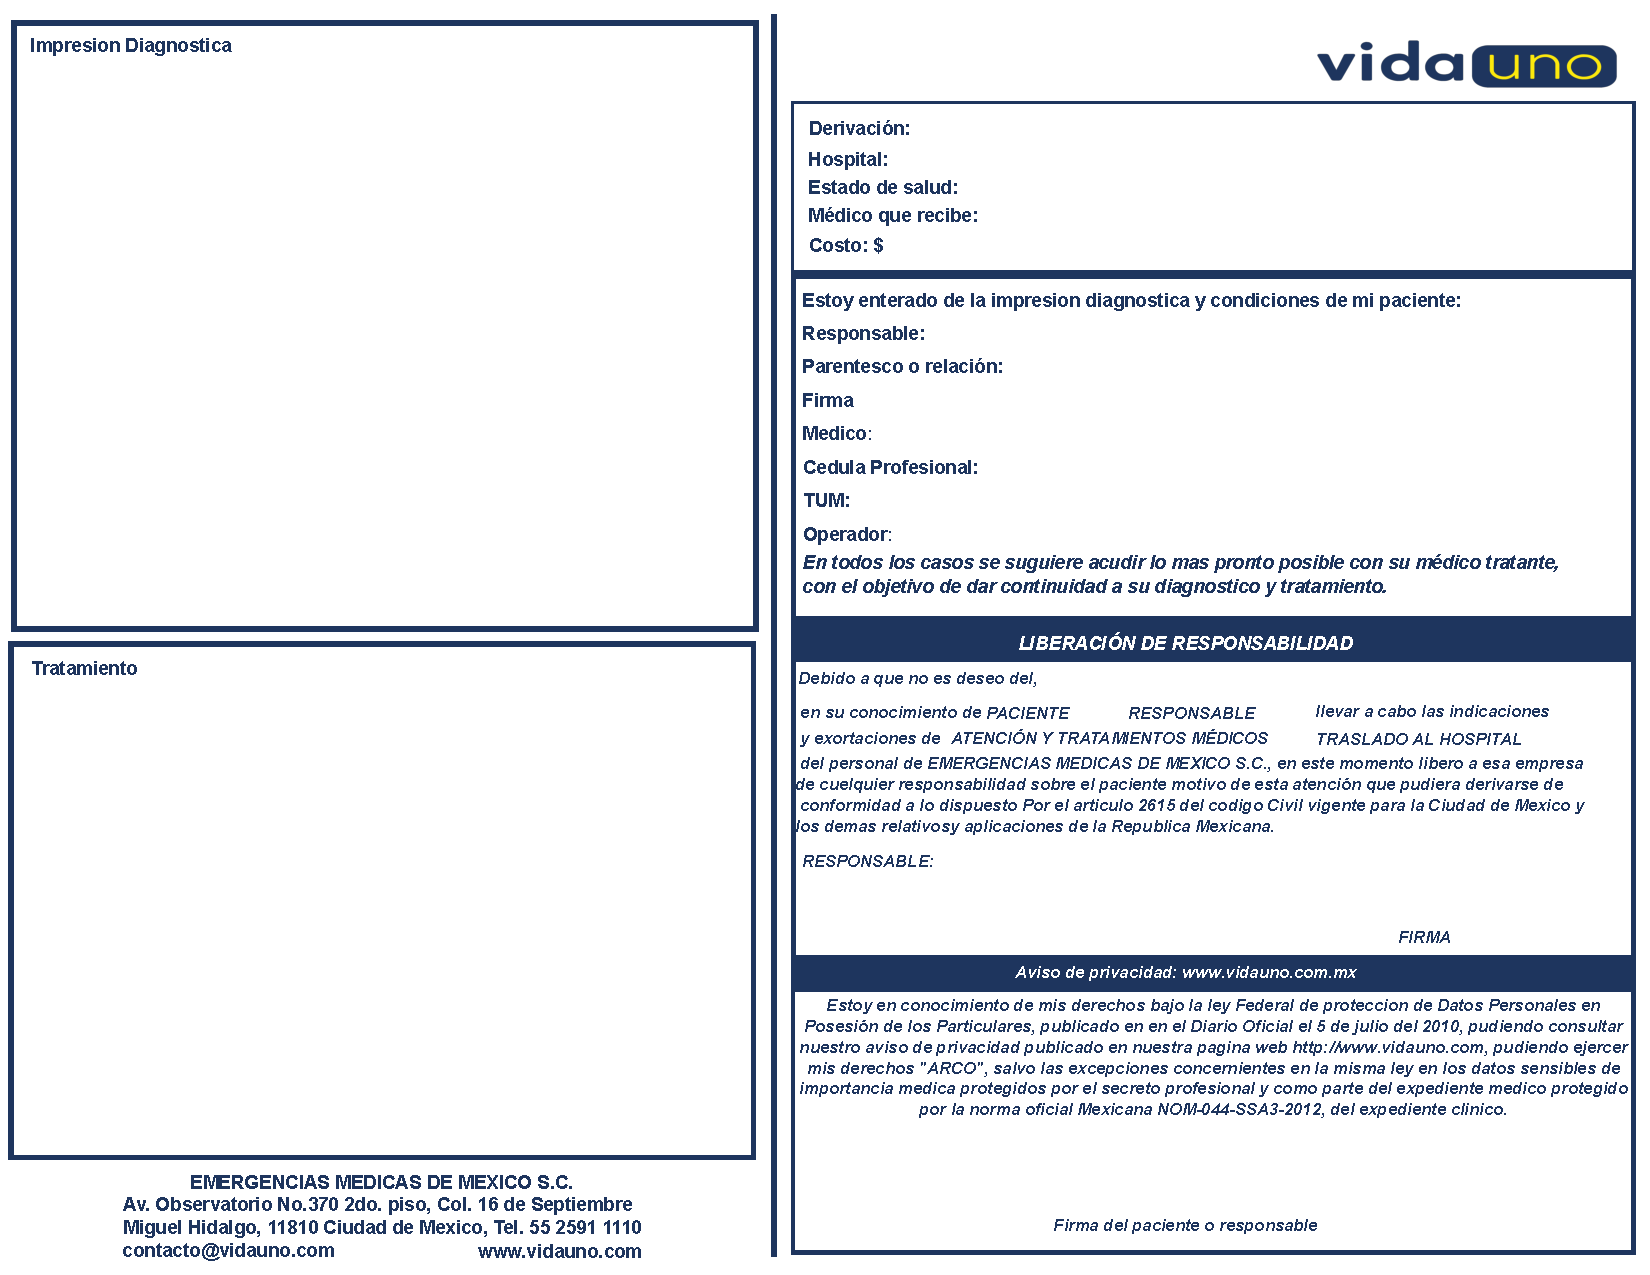
\includegraphics[width=\unitlength,page=1]{paperless_template_page_2}}%
    %Impresion diagnostica
    \put(0.02433222,0.72271027){\color[rgb]{0.11764706,0.20784314,0.36862745}\makebox(0,0)[lt]{\lineheight{1.25}\smash{\begin{tabular}[t]{l}\fontfamily{lmss}\selectfont {{content.treatment}}\end{tabular}}}}%
    %Tratamiento
    \put(0.02377709,0.34714045){\color[rgb]{0.11764706,0.20784314,0.36862745}\makebox(0,0)[lt]{\lineheight{1.25}\smash{\begin{tabular}[t]{l}\fontfamily{lmss}\selectfont {{content.diagnostic_impresion}}\end{tabular}}}}%
    %Derivacion
    \put(0.56751227,0.6911999){\color[rgb]{0.11764706,0.20784314,0.36862745}\makebox(0,0)[lt]{\lineheight{1.25}\smash{\begin{tabular}[t]{l}\fontfamily{lmss}\selectfont {{content.derivation_type}}\end{tabular}}}}%
    \put(0.56751227,0.6721787){\color[rgb]{0.11764706,0.20784314,0.36862745}\makebox(0,0)[lt]{\lineheight{1.25}\smash{\begin{tabular}[t]{l}\fontfamily{lmss}\selectfont {{content.derivation_hospital}}\end{tabular}}}}%
    \put(0.60035291,0.65502334){\color[rgb]{0.11764706,0.20784314,0.36862745}\makebox(0,0)[lt]{\lineheight{1.25}\smash{\begin{tabular}[t]{l}\fontfamily{lmss}\selectfont {{content.state_of_health}}\end{tabular}}}}%
    \put(0.60169212,0.63688865){\color[rgb]{0.11764706,0.20784314,0.36862745}\makebox(0,0)[lt]{\lineheight{1.25}\smash{\begin{tabular}[t]{l}\fontfamily{lmss}\selectfont {{content.derivation_recive}}\end{tabular}}}}%    
    \put(0.54544497,0.61971664){\color[rgb]{0.11764706,0.20784314,0.36862745}\makebox(0,0)[lt]{\lineheight{1.25}\smash{\begin{tabular}[t]{l}\fontfamily{lmss}\selectfont {{content.derivation_amount}}\end{tabular}}}}%
    %Finalizacion
    \put(0.57431346,0.56661945){\color[rgb]{0.11764706,0.20784314,0.36862745}\makebox(0,0)[lt]{\lineheight{1.25}\smash{\begin{tabular}[t]{l}\fontfamily{lmss}\selectfont {{content.demarcation_responsable}}\end{tabular}}}}%
    \put(0.6223905,0.54640692){\color[rgb]{0.11764706,0.20784314,0.36862745}\makebox(0,0)[lt]{\lineheight{1.25}\smash{\begin{tabular}[t]{l}\fontfamily{lmss}\selectfont {{content.demarcation_relation}}\end{tabular}}}}%
    \put(0.54203741,0.50578489){\color[rgb]{0.11764706,0.20784314,0.36862745}\makebox(0,0)[lt]{\lineheight{1.25}\smash{\begin{tabular}[t]{l}\fontfamily{lmss}\selectfont {{content.crew_medic}}\end{tabular}}}}%
    \put(0.59900976,0.48543641){\color[rgb]{0.11764706,0.20784314,0.36862745}\makebox(0,0)[lt]{\lineheight{1.25}\smash{\begin{tabular}[t]{l}\fontfamily{lmss}\selectfont {{content.crew_medic_id_card}}\end{tabular}}}}%
    \put(0.53065814,0.46522944){\color[rgb]{0.11764706,0.20784314,0.36862745}\makebox(0,0)[lt]{\lineheight{1.25}\smash{\begin{tabular}[t]{l}\fontfamily{lmss}\selectfont {{content.crew_tum}}\end{tabular}}}}%
    \put(0.55816754,0.44488927){\color[rgb]{0.11764706,0.20784314,0.36862745}\makebox(0,0)[lt]{\lineheight{1.25}\smash{\begin{tabular}[t]{l}\fontfamily{lmss}\selectfont {{content.crew_operator}}\end{tabular}}}}%
    \put(0.92413649,0.32194201){\color[rgb]{0.11764706,0.20784314,0.36862745}\makebox(0,0)[lt]{\lineheight{1.25}\smash{\begin{tabular}[t]{l}\textbf{\textit{ X4 }}\end{tabular}}}}%
    \put(0.65327278,0.35657174){\color[rgb]{0.11764706,0.20784314,0.36862745}\makebox(0,0)[lt]{\lineheight{1.25}\smash{\begin{tabular}[t]{l}\textbf{\textit{ X1 }}\end{tabular}}}}%
    \put(0.77324116,0.32194201){\color[rgb]{0.11764706,0.20784314,0.36862745}\makebox(0,0)[lt]{\lineheight{1.25}\smash{\begin{tabular}[t]{l}\textbf{\textit{ X3 }}\end{tabular}}}}%
    \put(0.76701121,0.33763243){\color[rgb]{0.11764706,0.20784314,0.36862745}\makebox(0,0)[lt]{\lineheight{1.25}\smash{\begin{tabular}[t]{l}\textbf{\textit{ X2 }}\end{tabular}}}}%
    %\put(0.66004404,0.33814317){\color[rgb]{0.11764706,0.20784314,0.36862745}\makebox(0,0)[lt]{\lineheight{1.25}\smash{\begin{tabular}[t]{l}\textbf{\textit{☑︎}}\end{tabular}}}}%


  \end{picture}
\endgroup%
\end{figure}


\end{document}
